\subsection{一一映射}\label{subsec:1-8}

看下面从集合 $A$ 到集合 $B$ 的映射(图\ref{fig:1-23}):

\begin{figure}[htbp]
    \centering
    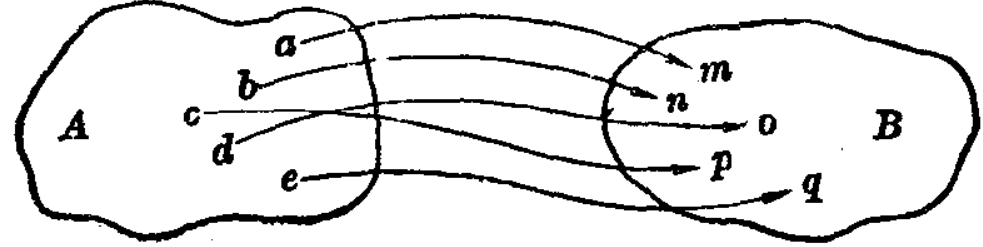
\includegraphics[width=0.7\textwidth]{../pic/1-23}
    \caption{}\label{fig:1-23}
\end{figure}

容易看出,这个映射有两个特点:第一,对于集合 $A$ 的不同元素,在集合 $B$ 中有不同的象;
第二,集合 $B$ 的每一个元素都是集合 $A$ 的某个元素的象,也就是说集合 $B$ 的每一个元素都有原象。

一般地,设 $A$,$B$ 是两个集合,$f: A \to B$ 是从集合 $A$ 到集合 $B$ 的映射,如果在这个映射
的作用下,对于集合 $A$ 中的不同元素,在集合 $B$ 中有不同的象,而且 $B$ 中每一个元素都有原象,
那么这个映射就叫做 \textbf{$A$ 到 $B$ 上的一一映射}。

例如,图 \ref{fig:1-23} 中的映射,就是 $A$ 到 $B$ 上的一一映射。又如:

(1)\mylabel{li:1-8-1} 设
\begin{align*}
    X &= \{1, 2, 3, 4, 5, \dots \},\\
    Y &= \{3, 5, 7, 9, 11, \dots \},
\end{align*}
取映射 $f: X \to Y$,使集合 $Y$ 中的元素 $y = 2x + 1$ 和集合 $X$ 中的元素 $x$ 对应。
这个映射是 $X$ 到 $Y$ 上的一一映射。

(2)把(1)中的 $Y$ 改为 $\{1, 3, 5, 7, 9, 11, \dots \}$,其他条件同(1)中一样,
那么这样得到的映射 $f': X \to Y$ 不是 $X$ 到 $Y$ 上的一一映射,因为这时 $Y$ 中的
元素 $1$ 没有原象。

(3)对于实数集 $R$,取映射 $f: R \to \buji{R^-}$,
\footnote{录注:甲种本原书中公式形如: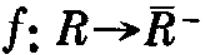
\includegraphics[width=1.8cm]{../pic/ch-1-8-1},注意补集符号的写法。}
使集合 $\buji{R^-}$ 中的元素 $y = x^2$ 和集合 $R$ 中的元素 $x$ 对应。这个映射不是 $R$ 到 $\buji{R^-}$ 上的一
一映射,因为 $R$ 中的不同元素 $2$ 与 $-2$ 在集合 $\buji{R^-}$ 中有同一个象 $4$。

(4)\mylabel{li:1-8-4} 对于(3)中的映射,如果改为映射 $f': \buji{R^-} \to \buji{R^-}$,使象集合
$\buji{R^-}$ 中的元素 $y = x^2$ 和原象集合 $\buji{R^-}$ 中的元素 $x$ 对应,那
么这个映射是 $\buji{R^-}$ 到 $\buji{R^-}$ 上的一一映射。

\lianxi

\begin{xiaotis}

\xiaoti{}

\begin{xiaoxiaotis}
    \vspace{-1.7em}
    \begin{minipage}{0.9\textwidth}
    \xiaoxiaoti{举出从集合 $A$ 到集合 $B$ 的映射的例子。}
    \end{minipage}
    
    \xiaoxiaoti{举出集合 $A$ 到集合 $B$ 上的一一映射的例子。}

    \xiaoxiaoti{映射与一一映射有什么相同和不同的地方?}
\end{xiaoxiaotis}

\xiaoti{习题二第3题的三个对应中,哪些是映射,哪些是一一映射?}

\xiaoti{在集合 $A$ 到集合 $B$ 上的一一映射中,}

\begin{xiaoxiaotis}
    \xiaoxiaoti{对于集合 $A$ 中的任意一个元素 $a$,在集合 $B$ 中是不是有象?是不是只有一个象?}

    \xiaoxiaoti{对于集合 $B$ 中的任意一个元素 $b$,在集合 $A$ 中是不是有原象?是不是只有一个原象?}
\end{xiaoxiaotis}

\xiaoti{下列各表分别表示从集合 $A$(元素 $a$)到集合 $B$(元素 $b$)的一个映射,
判断这些映射是不是 $A$ 到 $B$ 上的一一映射:}

\begin{xiaoxiaotis}
    
    \vspace{0.5em}
    \xiaoxiaoti{
        \begin{tabular}{|*{4}{w{c}{2em}|}}
            \hline
            $a$ & 2 & 3 & 4 \\
            \hline
            $b$ & 5 & 6 & 7 \\
            \hline
        \end{tabular}
    }
    
    \vspace{0.5em}
    \xiaoxiaoti{
        \begin{tabular}{|*{6}{w{c}{2em}|}}
            \hline
            $a$ & $0^\circ$ & $30^\circ$ & $60^\circ$ & $120^\circ$ & $150^\circ$ \\
            \hline
            \rule{0pt}{2em} $b$ & 0 & $\dfrac 1 2$ & $\dfrac{\sqrt 3} 2$ & $\dfrac{\sqrt 3} 2$ & $\dfrac 1 2$ \\[5pt]
            \hline
        \end{tabular}
    }

    \vspace{0.5em}
    \xiaoxiaoti{
        \begin{tabular}{|*{3}{w{c}{2em}|}}
            \hline
            $a$ & $a \in Q$ & $a \in \buji{Q}$ \\
            \hline
            $b$ & 1 & 0 \\
            \hline
        \end{tabular}
    }

\end{xiaoxiaotis}

\end{xiaotis}
